\documentclass[11pt]{beamer}
\title{Learning Loop Invariants for Program Verification}
\usepackage{verbatim}
\usepackage{amsmath}
\usepackage{amsthm}
\usepackage{graphics}
\usepackage{color}
\usepackage{stmaryrd}
\usepackage{multicol}

\newtheorem{proposition}{Proposition}

\date{\today}
\author{Xujie Si et al.}


\begin{document}
\maketitle
\begin{frame}\frametitle{Loop Invariant}
Hoare Triple: $\{P\}S\{Q\}$

Rule about loops in Hoare's logic:
\[\dfrac{P\Rightarrow I (pre), \{I\wedge B\}S\{I\} (inv), (I\wedge \neg B)\Rightarrow Q (post)}{\{P\}\texttt{while } B \texttt{ do } S \{Q\}}\]

\textbf{Loop Invariant Inference Problem}: given a pre-condition $P$ and a post-condition $Q$ and a program $S$ containing a single loop, can we find a predicate $I$ such that $\{P\}S\{Q\}$ is valid?

\textbf{Loop Invariant Inference Problem} is undecidable.

\end{frame}


\begin{frame}\frametitle{Loop Invariant: Example}
\begin{example}

\[x : = -50; \texttt{while } (x < 0) \texttt{ do }\]
\[\{x : = x + y; y := y + 1\} \texttt{ assert } (y > 0)\]

\end{example}
For the example loop above, it is easy to check $x < 0 \vee y > 0$ is a valid invariant.
\[x = -50 \rightarrow x < 0\vee y > 0\]
\[x < 0 \vee y > 0 \wedge x \ge 0 \rightarrow y > 0 \]
\end{frame}

\begin{frame}\frametitle{Idea}
The basic idea of this paper is to mimic how human experts reason the loop invariant.

\begin{example}
\begin{multicols}{2}
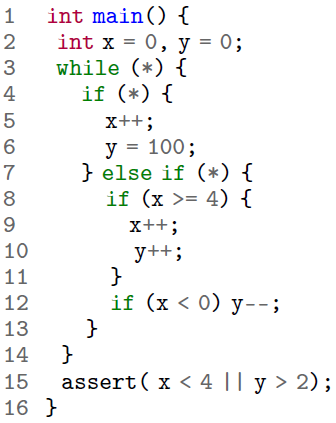
\includegraphics[scale = 0.45]{1.png}

\begin{itemize}
\item Start by reading the assertion. $x, y$.
\item $x$ may increase. $x < 4$ may not always hold.
\item How can $x \ge 4$: by executing the first branch $4$ times. Then we guess $y \ge 100$ because...
\item $x < 4 \vee y \ge 100$ is not enough, then add $x \ge 0$
\item $x \ge 0 \wedge (x < 4 \vee y \ge 100)$

\end{itemize}
\end{multicols}
\end{example}
\end{frame}

\begin{frame}\frametitle{Programming the Reasoning Procedure with NN}
\begin{itemize}
\item A structured external memory representation of the program.
\item Multi-step autoregressive model for incremental loop incariant construction.
\item An attention component that mimics the varying focus in each step.

\end{itemize}

\end{frame}

\begin{frame}\frametitle{Overall Framework}
\begin{center}
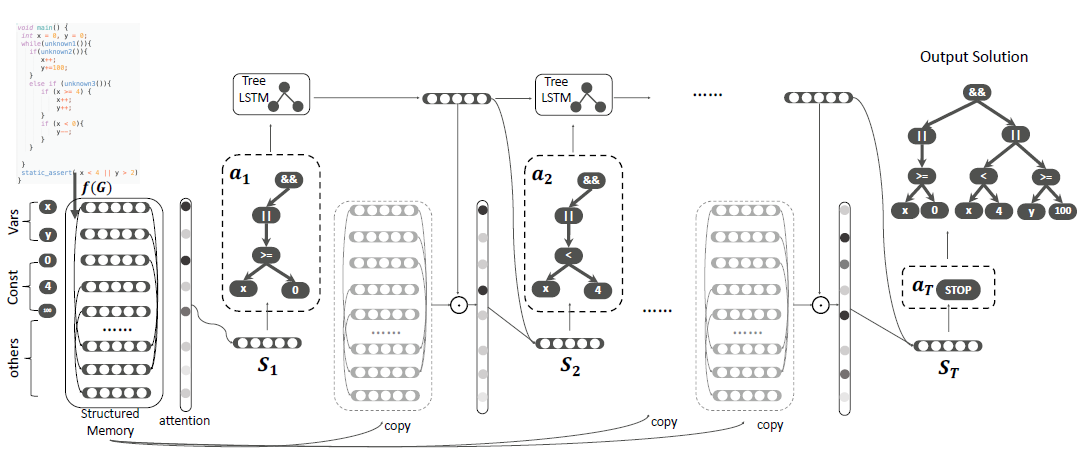
\includegraphics[scale = 0.39]{2.png}

\end{center}

\end{frame}

\begin{frame}\frametitle{Structured External Memory}
\begin{itemize}
\item First, convert a given program into a static single assignment form, then a flow graph where a vertex is an AST.

\item Then, convert the graph into vector representation. $E = \{(e_x^{(i)}, e_y^{(i)},e_t^{(i)})\}$.

\end{itemize}
\begin{center}

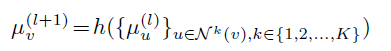
\includegraphics[scale = 0.4]{6.png}

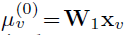
\includegraphics[scale = 0.4]{5.png}

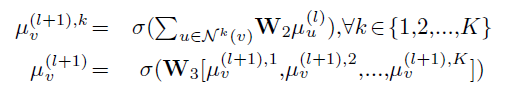
\includegraphics[scale = 0.4]{4.png}

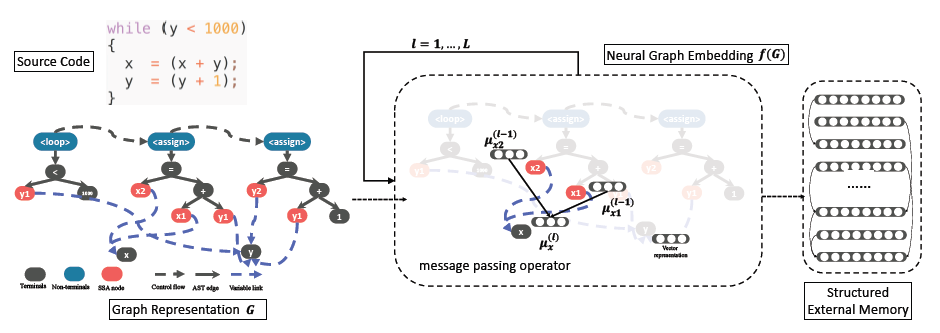
\includegraphics[scale = 0.4]{3.png}
\end{center}

\end{frame}

\begin{frame}\frametitle{Multi-Step Decision Making Process}
\begin{definition}[Loop Invariant]
We define the loop invariant to be a tree $\mathcal{T}$
\[\mathcal{T} = (\mathcal{T}_1 \vee \mathcal{T}_2\ldots) \wedge (\mathcal{T}_{t+1} \vee \mathcal{T}_{t+2}\ldots)\wedge \ldots \wedge (\ldots\mathcal{T}_{T - 1} \vee \mathcal{T}_{T})\]
\end{definition}

$T_t$ is $X < 2\times y + 10 - z$.

MDP: use MDP to model the problem of constructing the invariant incrementally.

$\mathcal{M}^G = (s_1, a_1, r_1, \ldots, s_T, a_T, r_T)$
\begin{itemize}
\item $a_t = (op_t, \mathcal{T}_t)$. $op_t$ can be $\wedge $ or $\vee $.
\item $s_t = (G, \mathcal{T}^{ < t})$.

\end{itemize}

\end{frame}

\begin{frame}\frametitle{Reward Design $r_t$}
\textbf{Early Reward}: the goal is to quickly remove the trivial and meaningless predicates. e.g. $e == e, e < e$. Examine partially generated $\mathcal{T}^t$.

\textbf{Continuous Reward}: $ce_{pre}, ce_{inv}, ce_{post}$ and $pass_{pre}, pass_{inv}, pass_{post}$.
No new counterexample is introduced: 
\begin{center}
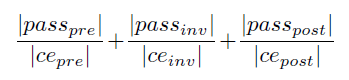
\includegraphics[scale = 0.4]{7.png}
\end{center}
New counterexample introduced: 
\begin{center}
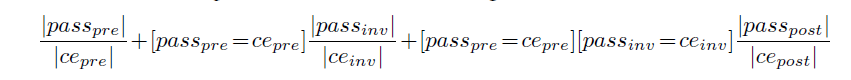
\includegraphics[scale=0.4]{8.png}

\end{center}
\end{frame}

\begin{frame}\frametitle{Training Objective and Expected Policy Reward}

\begin{center}
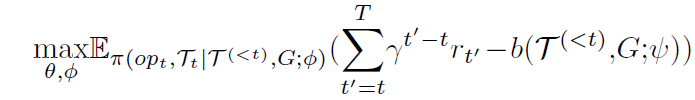
\includegraphics[scale=0.4]{9.png}

\end{center}
\end{frame}

\begin{frame}\frametitle{Termination}
Situations for termination:
\begin{itemize}
\item Successfully generated.
\item The tree of the generated invariant reach a ceiling number of branches.
\item The agent generate invalid action.

\end{itemize}

\end{frame}
\begin{frame}\frametitle{Experiment Result}

\begin{center}

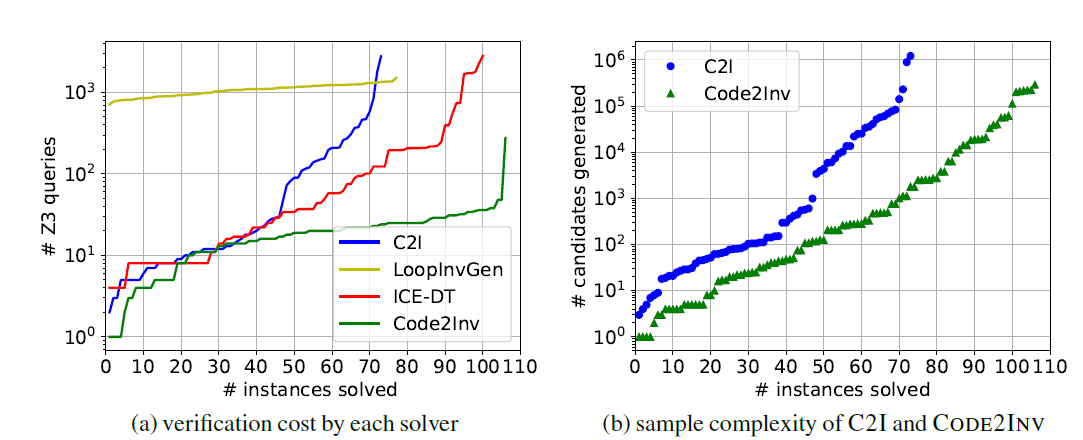
\includegraphics[scale = 0.35]{10.png}
\end{center}

\end{frame}
\end{document}